\documentclass{article}

\usepackage{amsmath} % math stuff
\usepackage{amssymb} % math stuff
\usepackage{array} % equations and stuff
\usepackage{bm} % bold math
%\usepackage{caption} % suppressed table numbering; incompatible with revtex, and longtable, I think
\usepackage{comment} % comment environment
%\usepackage{enumitem} % customization of enumeration, itemize, and description
\usepackage[T1]{fontenc} % font encoding for special characters, must also use scalable font package
\usepackage[margin=0.8in]{geometry} % paper sizes and margins (but be careful not to mess up pre-defined pages)
\usepackage{graphicx} % for graphics
%\usepackage{helvet} % default font is the helvetica postscript font
\usepackage{layouts} % print units like widths
\usepackage{lipsum} % lorem ipsum filler text
\usepackage{lmodern} % scalable font?
\usepackage{longtable} % multi-page tables
\usepackage{makecell} % specify line-breaks in table cells
\usepackage{mathrsfs} % math script font
\usepackage{mhchem} % easier chemical formula
\usepackage{microtype} % allows disabling of ligatures
%\usepackage{newcent} % new century schoolbook font
\usepackage{nicefrac}
\usepackage{numprint} % print and format (large) numbers
\usepackage{parskip} % removes paragraph indentation, and adjusts paragraph skip, as well as list items
\usepackage{pdfpages} % add pdf files as pages
%\usepackage{setspace} % adjust text spacing and indents
\usepackage{siunitx} % decimal alignment
\usepackage{subfigure} % divided figures
%\usepackage{tabu} % extra table options
\usepackage{textcomp} % symbols
\usepackage{threeparttablex} % better footnotes with longtable
\usepackage{titling} % title placement
\usepackage{ulem} % strikethrough text
%\usepackage{url} % superceded by hyperref
\usepackage{verbatim} % verbatim environment
\usepackage{xcolor} % colors and color boxes
\usepackage{xspace} % commands that don't eat up white space
\usepackage{hyperref} % links and page setup; should always come last

\hypersetup{
 bookmarks=true,
 colorlinks=true,
 citecolor=blue,
 linkcolor=blue,
 urlcolor=blue,
 pdfstartview={XYZ null null 1.0} % default open view is 100%
}

\DisableLigatures[f,t]{encoding = T1} % disable ff, fi, fl, tt ligatures, without f option, it also disables -- = endash
\renewcommand{\arraystretch}{2.0} % extra vertical space in tables

\begin{document}

\pagestyle{empty} % don't number pages

% custom title
\begin{center}
{\LARGE Classic Riddler}

\vspace{0.15in}

{\Large 6 September 2019}
\end{center}


\section*{Riddle:}

Suppose you're playing a match at the U.S. Open, and you're slightly better than the competition: your chances of winning any given point are exactly 55 percent.
(Yes, most players are more likely to win the points they serve, but we're simplifying things a bit.)
What are your chances of winning a three-set match, as played by the women, or a five-set match, as played by the men?
And what are your chances of winning the whole tournament (seven consecutive matches)?

If you're not familiar with the scoring system in tennis, you can read \href{https://www.usta.com/en/home/improve/tips-and-instruction/national/tennis-101--scoring.html}{more about it here}.
In short, the first to 4 points wins a game (as long as they've won 2 more points than their opponent), the first to six games wins a set (as long as they've won two more games), and the first to two sets (for women) or three sets (for men) wins the match.
If at any point a set is tied at six games apiece, that set is decided by a tiebreaker, in which the first to 7 points wins (with the same 2-point margin rule applying here).

You know, I thought tennis scoring was pretty straightforward until I had to write it down.


\section*{Solution:}

I set up this problem as a tree with interconnected probabilities.
The tree for a single game is shown on the next page.
Each state is a score, and there is a probability for each state that is the probability to win starting from that state.
The probabilities are determined by the two outcomes after each state: winning the point with probability $p$, and losing the point with probability $1-p$.
For this riddle $p=0.55$.
The probabity of winning at state W is 1, and the probability of winning at state L is 0.
The other probabilities can be solved by a series of iterated equations.

The calculation starts with the three states at the bottom, $P(40-40)$, $P(\rm{Ad\ in})$, and $P(\rm{Ad\ out})$, which are described as follows:

\[
P(40-40)=pP(\rm{Ad\ in})+(1-p)P(\rm{Ad\ out})
\]
\[
P(\rm{Ad\ in})=pP(\rm{W})+(1-p)P(40-40)
\]
\[
P(\rm{Ad\ out})=pP(40-40)+(1-p)P(\rm{L})
\]

Solving gives the initial (approximate) solutions $P(40-40)=0.599$, $P(\rm{Ad\ in})=0.8196$, and $P(\rm{Ad\ out})=0.3295$.
The remaining probabilities are solved bottom-to-top with similar equations.

This kind of iterated equation solving is perfect for spreadsheet calculations, which I have done in the file \texttt{tennis.xlsx}\,.
The first part of the spreadsheet solves both the tiebreak and the game based on winning individual points.
The probability of winning a game is mathematically equivalent to the probability of winning a tiebreak starting from a score of 3-3.
The spreadsheet shows that the probability of winning any game is (approximately) 0.6231, and for a tiebreak is (approximately) 0.6542.

These numbers are then used in the spreadsheet to make a similar calculation for winning a set.
The overall probability of winning a set is therefore (approximately) 0.815.

The final portion of the spreadsheet then calculates the probability of winning a womens match and tournament, and a mens match and tournament, which are the final solutions.
I list all the combinations of sets which lead to a match win in both cases, and add up the individual probabilities to get the final number.
This is then raised to the seventh power to get the total probability of winning each tournament.
The probability of winning a womens match and tournament, respectively, are (approximately)
\fcolorbox{red}{white}{\bf91.0\% and 51.7\%}\,,
and the probability of winning a mens match and tournament, respectively, are (approximately)
\fcolorbox{red}{white}{\bf95.3\% and 71.4\%}\,.

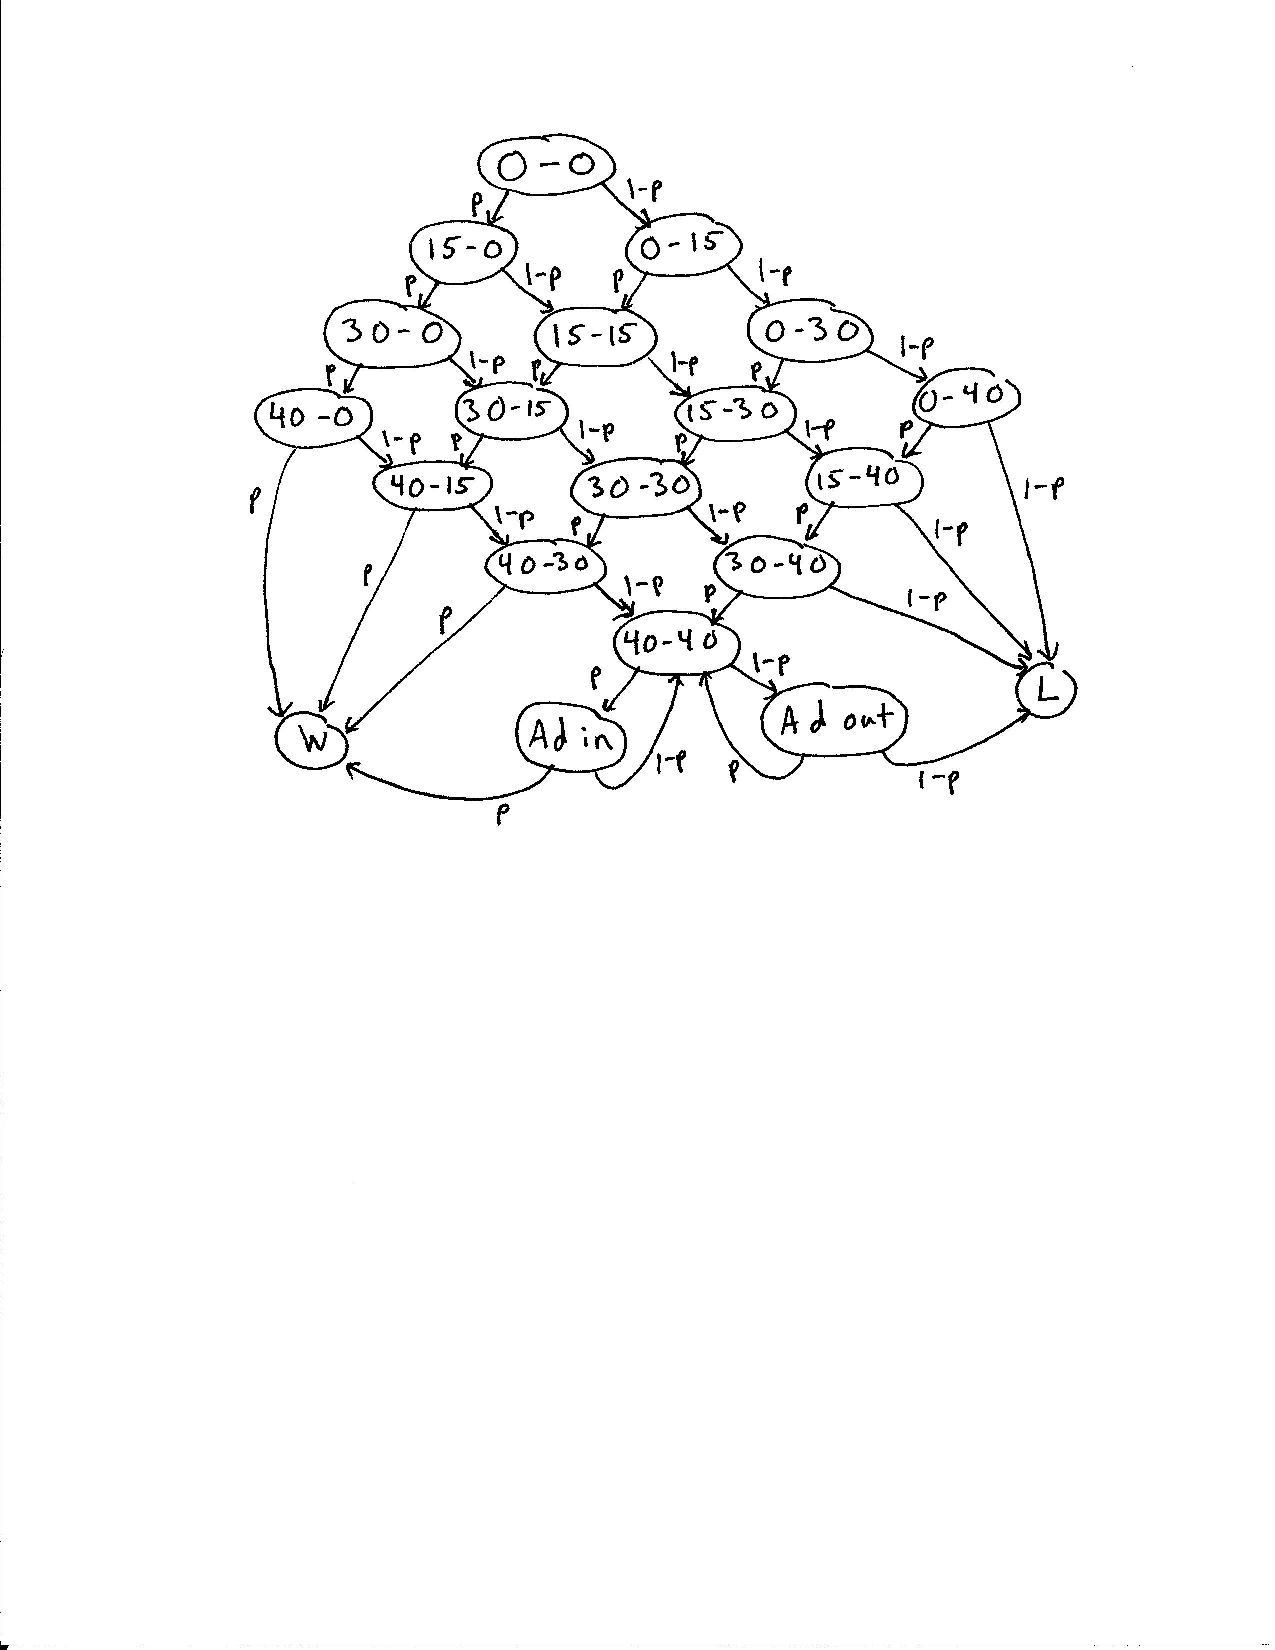
\includepdf{game_tree_scan.pdf}

\end{document}